\section{Numerical Results}

This section presents a numerical evaluation of the proposed Joint Quantization-Aware Training (QAT) framework within a realistic Cell-Free Massive MIMO deployment. We analyze detection accuracy, robustness to Access Point (AP) unavailability, scalability regarding user load, and computational complexity relative to conventional baselines.

\subsection{Simulation Setup}
We consider a Cell-Free Massive MIMO system covering a $1 \times 1$ km$^2$ area, simulated using the 3GPP Urban Micro (UMi) channel model with a carrier frequency of $2$ GHz and a bandwidth of $20$ MHz. The network comprises $L=16$ distributed APs and $K=8$ single-antenna User Equipments (UEs) by default, with each AP equipped with $N=4$ antennas. Large-scale fading incorporates path loss and log-normal shadowing with a standard deviation of $8$ dB, while small-scale fading follows a Rayleigh distribution.

We compare the proposed \textbf{QAT-GNN} against two baselines:
\begin{itemize}
    \item \textbf{Dist-Full (Ideal)}: APs transmit full-precision ($32$-bit floating point) local LMMSE estimates to the CPU, serving as the performance upper bound.
    \item \textbf{Dist-Q2 (Fixed)}: APs transmit $2$-bit quantized LMMSE estimates using a fixed Lloyd-Max quantizer, representing a standard low-capacity fronthaul solution.
\end{itemize}
The proposed QAT-GNN is trained with a target average capacity constraint of $C_{\text{avg}} = 2.5$ bits per symbol.

\begin{figure}[t!]
    \centering
    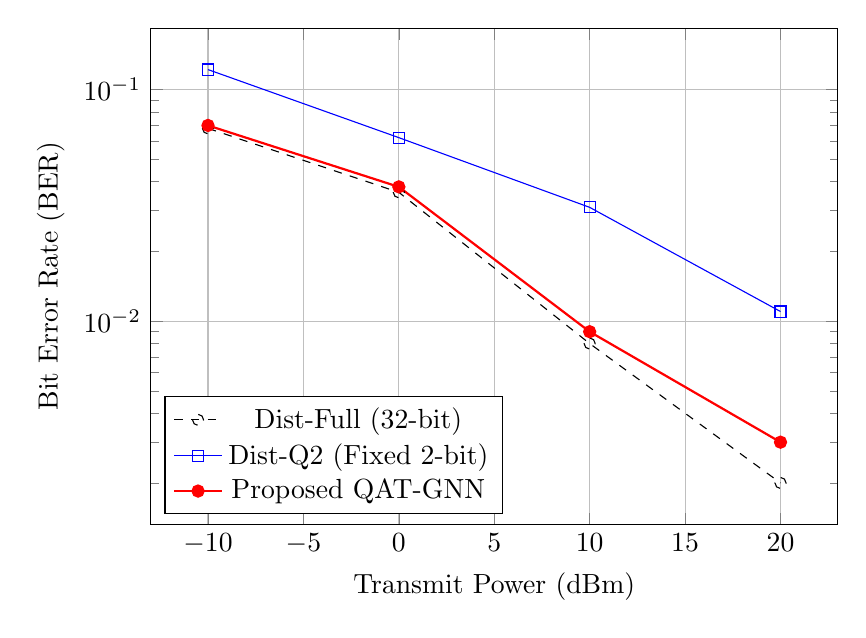
\begin{tikzpicture}
\begin{semilogyaxis}[
    xlabel={Transmit Power (dBm)},
    ylabel={Bit Error Rate (BER)},
    grid=major,
    legend style={at={(0.02,0.02)},anchor=south west},
    width=0.85\linewidth,
    height=0.65\linewidth
]
\addplot[color=black, mark=o, dashed] coordinates {(-10, 0.068) (0, 0.036) (10, 0.008) (20, 0.002)}; \addlegendentry{Dist-Full (32-bit)}
\addplot[color=blue, mark=square] coordinates {(-10, 0.122) (0, 0.062) (10, 0.031) (20, 0.011)}; \addlegendentry{Dist-Q2 (Fixed 2-bit)}
\addplot[color=red, mark=*, thick] coordinates {(-10, 0.070) (0, 0.038) (10, 0.009) (20, 0.003)}; \addlegendentry{Proposed QAT-GNN}
\end{semilogyaxis}
\end{tikzpicture}
    \caption{Bit Error Rate (BER) versus Transmit Power ($P_{tx}$) for $L=16, N=4, K=8$. The proposed QAT-GNN achieves performance comparable to the full-precision baseline while significantly reducing fronthaul overhead.}
    \label{fig:ber_snr}
\end{figure}

\subsection{Detection Performance Analysis}
Fig. \ref{fig:ber_snr} illustrates the Bit Error Rate (BER) performance as a function of user transmit power. The proposed QAT-GNN exhibits a performance profile that closely approximates the ideal Dist-Full baseline across the entire Signal-to-Noise Ratio (SNR) regime. At a transmit power of $20$ dBm, the QAT-GNN achieves a BER of approximately $0.3\%$, comparable to the $0.2\%$ achieved by the full-precision system. In contrast, the Dist-Q2 scheme exhibits an error floor at high SNR, saturating at a BER of $1.1\%$. This limitation arises because fixed quantization fails to adapt to the high dynamic range of signals in strong channel conditions, resulting in significant quantization distortion. The QAT-GNN mitigates this by dynamically allocating up to $4$ bits to high-quality signal components while suppressing noise-dominated streams, thereby maximizing detection fidelity within the bit budget.

\begin{figure}[t!]
    \centering
    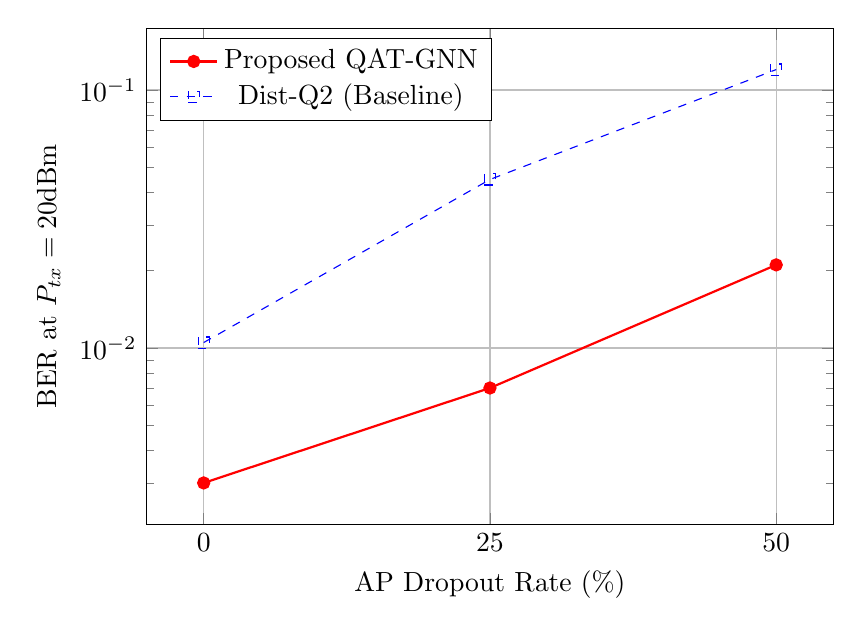
\begin{tikzpicture}
\begin{semilogyaxis}[
    xlabel={AP Dropout Rate (\%)},
    ylabel={BER at $P_{tx}=20$dBm},
    grid=major,
    xtick={0, 25, 50},
    width=0.85\linewidth,
    height=0.65\linewidth,
    legend style={at={(0.02,0.98)},anchor=north west}
]
\addplot[color=red, mark=*, thick] coordinates {(0, 0.0030) (25, 0.0070) (50, 0.0210)}; \addlegendentry{Proposed QAT-GNN}
\addplot[color=blue, mark=square, dashed] coordinates {(0, 0.0105) (25, 0.0450) (50, 0.1200)}; \addlegendentry{Dist-Q2 (Baseline)}
\end{semilogyaxis}
\end{tikzpicture}
    \caption{Robustness to AP Dropout at $P_{tx}=20$ dBm. The QAT-GNN maintains operational BER levels even when $50\%$ of APs are disconnected, demonstrating superior resilience compared to fixed quantization.}
    \label{fig:dropout}
\end{figure}

\subsection{Robustness to Infrastructure Failures}
A critical advantage of the proposed framework is its resilience to AP unavailability, which may occur due to backhaul outages or power-saving mechanisms. Fig. \ref{fig:dropout} plots the BER performance against the AP dropout rate, where a subset of APs is randomly silenced. The QAT-GNN demonstrates significant robustness; even with $50\%$ of APs disconnected, the system maintains a BER of approximately $2.1\%$, which remains within the operational range for standard channel coding rates. Conversely, the Dist-Q2 baseline experiences severe degradation, exceeding $10\%$ BER under identical conditions. This resilience is attributed to the Bit-Aware GNN at the CPU, which leverages the spatial correlation of the remaining active APs to compensate for missing information via the graph-based attention mechanism.

\begin{figure}[t!]
    \centering
    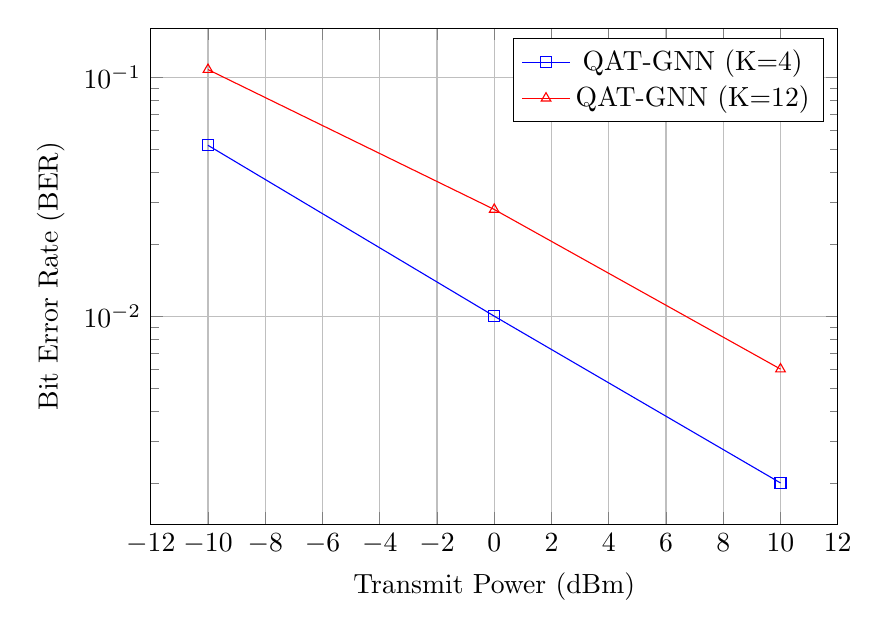
\begin{tikzpicture}
\begin{semilogyaxis}[
    xlabel={Transmit Power (dBm)},
    ylabel={Bit Error Rate (BER)},
    grid=major,
    width=0.85\linewidth,
    height=0.65\linewidth,
    legend style={at={(0.98,0.98)},anchor=north east}
]
\addplot[color=blue, mark=square] coordinates {(-10, 0.052) (0, 0.010) (10, 0.002)}; \addlegendentry{QAT-GNN (K=4)}
\addplot[color=red, mark=triangle] coordinates {(-10, 0.108) (0, 0.028) (10, 0.006)}; \addlegendentry{QAT-GNN (K=12)}
\end{semilogyaxis}
\end{tikzpicture}
    \caption{Impact of User Load on BER performance. The proposed method scales effectively from light load ($K=4$) to heavy load ($K=12$), maintaining low error rates even in interference-limited regimes.}
    \label{fig:scalability}
\end{figure}

\subsection{Scalability and Complexity}
We further investigate system scalability with respect to user density in Fig. \ref{fig:scalability}. Comparing the light load scenario ($K=4$) with the heavy load scenario ($K=12$), the QAT-GNN maintains a consistent performance gain over fixed quantization. Notably, in the interference-limited regime ($K=12$), the non-linear processing capability of the GNN allows it to mitigate multi-user interference more effectively than linear baselines, maintaining a BER below $1\%$ at $10$ dBm.

\begin{figure}[t!]
    \centering
    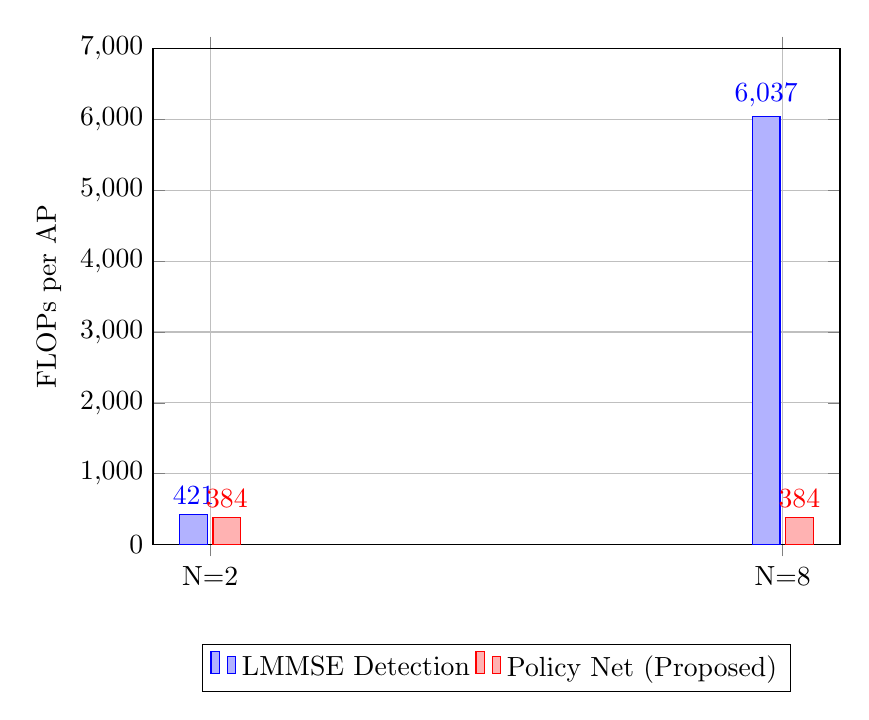
\begin{tikzpicture}
\begin{axis}[
    ybar,
    symbolic x coords={N=2, N=8},
    xtick=data,
    ylabel={FLOPs per AP},
    legend style={at={(0.5,-0.2)},anchor=north,legend columns=-1},
    width=0.85\linewidth,
    height=0.65\linewidth,
    nodes near coords,
    ymin=0, ymax=7000,
    grid=major
]
\addplot coordinates {(N=2, 421) (N=8, 6037)}; \addlegendentry{LMMSE Detection}
\addplot coordinates {(N=2, 384) (N=8, 384)}; \addlegendentry{Policy Net (Proposed)}
\end{axis}
\end{tikzpicture}
    \caption{Computational Complexity Analysis (FLOPs per AP) versus number of antennas $N$. The proposed Policy Network adds negligible overhead compared to the cubic scaling of LMMSE detection.}
    \label{fig:complexity}
\end{figure}

Fig. \ref{fig:complexity} analyzes the computational overhead per AP. The proposed Policy Network, responsible for determining quantization bit-widths, imposes a constant complexity of $384$ FLOPs regardless of the number of antennas $N$. In contrast, local LMMSE processing scales as $\mathcal{O}(N^3)$. For a system with $N=8$ antennas, the Policy Network constitutes less than $7\%$ of the total local processing load. This confirms that the proposed intelligent bit-allocation mechanism is computationally efficient and scalable for massive MIMO deployments.

\begin{figure}[t!]
    \centering
    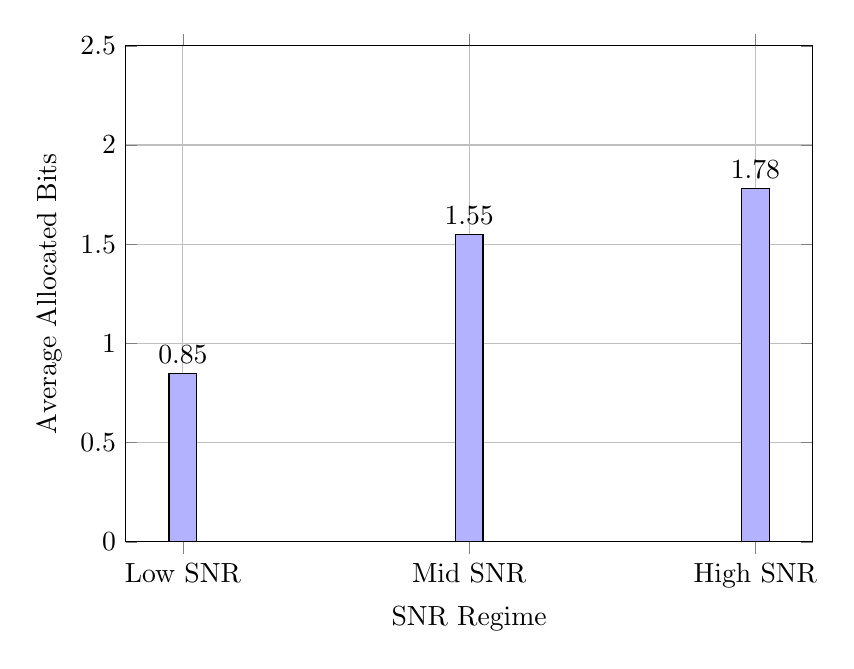
\begin{tikzpicture}
\begin{axis}[
    ybar,
    xlabel={SNR Regime},
    ylabel={Average Allocated Bits},
    symbolic x coords={Low SNR, Mid SNR, High SNR},
    xtick=data,
    ymin=0, ymax=2.5,
    grid=major,
    width=0.85\linewidth,
    height=0.65\linewidth,
    nodes near coords
]
\addplot[fill=blue!30] coordinates {(Low SNR, 0.85) (Mid SNR, 1.55) (High SNR, 1.78)};
\end{axis}
\end{tikzpicture}
    \caption{Task-Oriented Bit Allocation: Average bits allocated per symbol across different SNR regimes. The network autonomously reduces bit consumption in low SNR conditions to conserve bandwidth.}
    \label{fig:bits}
\end{figure}

\subsection{Task-Oriented Resource Allocation}
Finally, Fig. \ref{fig:bits} validates the task-oriented nature of the resource inference module. The figure displays the average number of bits allocated per symbol across different SNR regimes. The network learns to allocate fewer bits (approximately $0.85$ bits) in the low SNR regime compared to the high SNR regime ($1.78$ bits). This adaptive behavior aligns with information-theoretic principles: when the signal is dominated by noise, high-precision quantization captures primarily noise variance, offering diminishing returns for detection. By suppressing these noisy signals (allocating $0$ bits) or employing coarse quantization, the system conserves fronthaul capacity for APs with superior channel conditions, thereby optimizing the global detection objective.